% Options for packages loaded elsewhere
\PassOptionsToPackage{unicode}{hyperref}
\PassOptionsToPackage{hyphens}{url}
%
\documentclass[
  11pt,
]{article}
\usepackage{amsmath,amssymb}
\usepackage{iftex}
\ifPDFTeX
  \usepackage[T1]{fontenc}
  \usepackage[utf8]{inputenc}
  \usepackage{textcomp} % provide euro and other symbols
\else % if luatex or xetex
  \usepackage{unicode-math} % this also loads fontspec
  \defaultfontfeatures{Scale=MatchLowercase}
  \defaultfontfeatures[\rmfamily]{Ligatures=TeX,Scale=1}
\fi
\usepackage{lmodern}
\ifPDFTeX\else
  % xetex/luatex font selection
\fi
% Use upquote if available, for straight quotes in verbatim environments
\IfFileExists{upquote.sty}{\usepackage{upquote}}{}
\IfFileExists{microtype.sty}{% use microtype if available
  \usepackage[]{microtype}
  \UseMicrotypeSet[protrusion]{basicmath} % disable protrusion for tt fonts
}{}
\makeatletter
\@ifundefined{KOMAClassName}{% if non-KOMA class
  \IfFileExists{parskip.sty}{%
    \usepackage{parskip}
  }{% else
    \setlength{\parindent}{0pt}
    \setlength{\parskip}{6pt plus 2pt minus 1pt}}
}{% if KOMA class
  \KOMAoptions{parskip=half}}
\makeatother
\usepackage{xcolor}
\usepackage[margin=1in]{geometry}
\usepackage{graphicx}
\makeatletter
\def\maxwidth{\ifdim\Gin@nat@width>\linewidth\linewidth\else\Gin@nat@width\fi}
\def\maxheight{\ifdim\Gin@nat@height>\textheight\textheight\else\Gin@nat@height\fi}
\makeatother
% Scale images if necessary, so that they will not overflow the page
% margins by default, and it is still possible to overwrite the defaults
% using explicit options in \includegraphics[width, height, ...]{}
\setkeys{Gin}{width=\maxwidth,height=\maxheight,keepaspectratio}
% Set default figure placement to htbp
\makeatletter
\def\fps@figure{htbp}
\makeatother
\setlength{\emergencystretch}{3em} % prevent overfull lines
\providecommand{\tightlist}{%
  \setlength{\itemsep}{0pt}\setlength{\parskip}{0pt}}
\setcounter{secnumdepth}{5}
\usepackage{booktabs}
\usepackage{pdflscape}
\usepackage{tocloft}
\ifLuaTeX
  \usepackage{selnolig}  % disable illegal ligatures
\fi
\IfFileExists{bookmark.sty}{\usepackage{bookmark}}{\usepackage{hyperref}}
\IfFileExists{xurl.sty}{\usepackage{xurl}}{} % add URL line breaks if available
\urlstyle{same}
\hypersetup{
  pdftitle={Cluster analysis of nearshore physical predictors},
  pdfauthor={Edward Gregr},
  hidelinks,
  pdfcreator={LaTeX via pandoc}}

\title{Cluster analysis of nearshore physical predictors}
\author{Edward Gregr}
\date{September 14, 2024}

\begin{document}
\maketitle

{
\setcounter{tocdepth}{2}
\tableofcontents
}
\listoffigures

\listoftables
\newpage

\hypertarget{introduction}{%
\section{Introduction}\label{introduction}}

Relatively little is known about nearshore benthic habitat types and
associated marine benthic invertebrate and algal communities along the
BC coast, as much of the work by DFO is focused on species of commercial
interest. Benthic habitat types and community composition of the
nearshore region represent data gaps that need to be addressed to
provide scientific support to marine use planning initiatives. In the
absence of an empirical representation for data-poor species, there is a
need to have a proxy representing areas of similar environmental
conditions to use as a framework to collate existing information on the
distribution of kelp and other nearshore benthic species.

The key deliverable for this project is a method, including supporting R
scripts, to generate clusters representing areas of common environmental
conditions from existing spatial layers. Deliverables will include the
resulting spatial clusters with appropriate metadata, and a
well-documented R script used to create the layers.

Examples of clusters are generated across two spatial extents: The full
Queen Charlotte Strait (QCS) `data' region, and a reduced area with
higher data quality. These are included to illustrate the results and
some of the challenges with unsupervised classification. The scripts
include an RMarkdown file which produces a PDF report of the results.
This allows for efficient comparisons of different cluster formulations.

The clustering scripts rely on TIF files provided by the Marine Spatial
Ecology \& Analysis (MSEA) section. The code assumes the TIFs are in the
same project, but imposes a common resolution and extent to ensure all
inputs have identical spatial configurations.

\hypertarget{background}{%
\subsection{Background}\label{background}}

Following the methods of Mora-Soto et al.~2024, create a k-means
clustering of biophysical layers to support the representation of
potential kelp extents and habitat types in British Columbia.

\hypertarget{k-means-classification}{%
\subsection{K-means classification}\label{k-means-classification}}

Standard K-means clustering works by minimizing the Euclidean distance
between data points and cluster centroids. It is designed for continuous
numeric data, and is described as sensitive to the `shape' of those data
(e.g., range, distribution). Much attention was therefore paid to
outliers and skewness. All predictors were transformed if warranted,
then centered and scaled to ensure all predictors contribute equally.

Euclidean distance also means that k-means will strive for clusters of
uniform in size, is very sensitive to outliers, assumes that data points
in each cluster form a sphere around each centroid (KDnuggets 2024).
Categorical variables cannot be directly used in standard K-means
clustering as they do not have a meaningful Euclidean distance. While
methods for mixed data exist (e.g., in the R cluster package), the
clustering on non-Euclidean distances is more time consuming. Thus,
these methods have limits on the size of the data (e.g., the pam()
algorithm is limited to 65,000 observations). Given that the QCS study
area contains over 17,000,000 valid pixels structuring a re-sampling
analysis using these tools was deemed out of scope. Guidance on
selecting the appropriate number of clusters include examining the
within sum of squares, average silhouette width, gap analysis, and the
separation of the clusters (via Principal Component Analysis). Cluster
analysis can be open-ended if there are no data for validation given
that results can vary with the different data sets included and the
number of clusters.

\hypertarget{data-preparation}{%
\section{Data preparation}\label{data-preparation}}

In discussions with the Project Manager, the layers of interest (Table
1) were chosen to reflect the best available coast-wide coverage at a
resolution of 20x20 m2. Recent work on classifying substrate (Gregr et
al.~2020) and species distribution (Nephin et al.~2016) has been based
on this spatial framework, and the various layers are regularly updated
by DFO. The data were provided by DFO as TIF files and were loaded
directly into R. Rasters are all assumed to have the same projection and
resolution. As part of the data loading process, the rasters are
standardized to the combined minimum spatial extents to resolve any
differences in spatial extents. The coastwide Sentinel SST data were
re-sampled onto the same spatial reference. Following Barbosa et al.,
unsuitable depths are removed from the source data. Not only is this
critical for the bathymetry-based roughness layers (as the bathymetry
includes upland areas), it also focuses the clustering on the photic
zone. Bathymetry was then dropped as a classifying predictor. Since
clustering is only done for compete cases, this restriction defines the
extent of the classification.

\hypertarget{description-of-predictors}{%
\subsection{Description of predictors}\label{description-of-predictors}}

\begin{table}
\centering
\caption{\label{tab:DescripTable}Description of the predictors considered and the processes they represent}
\centering
\begin{tabular}[t]{p{1in}p{1in}p{3in}}
\toprule
Process & Predictor & Description\\
\midrule
Light, Energy & bathymetry & Kelps are light-restricted, so depth is crucial for forming clusters in the photic zone. Following Barbosa et al., bathymetry was used to restrict the study to suitable depths, rather than as a classifying variable.\\
Bottom type & substrate & As kelp holdfasts must be attached to hard substrates, a description of bottom type is an essential characteristic of kelp habitat suitability. We used the substate predictions (Mud, Sand, Mixed, and Hard) from Gregr et al. (2019), updated by MSEA to include the relative exposure index (instead of fetch).\\
Roughness & std\_dev\_slope, arc-chord rugosity & Roughness\\
Circulation & circ\_mean\_summer, tidal\_mean\_summer & The predictor circ\_mean is intended proxy for larger water mass movements, while tidal\_mean is a representation of diurnal and fortnight tidal ranges.\\
Salinity & freshwater\_index, salt\_mean\_summer, salt\_range & Kelps do better in higher salinity waters, as salinity tends to be correlated with both cooler temperatures and increased nutrients. We used a simple diffusion model developed by MSEA which shows potentially low salinity areas based on point estimates of riverine input (from the BC Freshwater Atlas).\\
\addlinespace
Relative exposure index & rei & In addition to influencing substrate, exposure is also an indicator of mixing and can also influence zoospore settlement. This updated relative exposure index (REI) from MSEA includes depth attenuated wave action combined with fetch and dominant winds.\\
Temperature & sentinel\_max,sentinel\_mean, sentinel\_sd, temp\_mean\_summer,temp\_range & Temperature ...\\
\bottomrule
\end{tabular}
\end{table}

\hypertarget{preliminary-predictor-assessment}{%
\section{Preliminary predictor
assessment}\label{preliminary-predictor-assessment}}

The loaded Raster stack is 4937 by 9684, giving a total of 47809908
pixels in the study domain. Much of this area is land, or deeper waters
excluded by the bathymetry.

The loaded data were examined for Skewness of the predictors

\begin{table}[!h]
\centering
\caption{\label{tab:SkewTable}Skewness values for selected, Transformed predictors.}
\centering
\begin{tabular}[t]{lr}
\toprule
  & x\\
\midrule
rei\_qcs & 1.9053617\\
salinity\_mean\_summer & -2.0837087\\
standard\_deviation\_slope & 0.5072371\\
temp\_range & 1.8629115\\
tidal\_mean\_summer & 1.0099057\\
\addlinespace
sst\_sentinel\_20m\_bi\_max & 0.5223937\\
\bottomrule
\end{tabular}
\end{table}

Examine correlations across predictors, and identify those beyond a
threshold of 0.6.

\begin{landscape}\begin{table}
\centering
\caption{\label{tab:Correlations}Correlation matrix for assessing predictor cross-correlations}
\centering
\resizebox{\ifdim\width>\linewidth\linewidth\else\width\fi}{!}{
\begin{tabular}[t]{lrrrrrrrrrrrrrr}
\toprule
  & bathymetry & circ\_mean\_summer & qcs\_freshwater\_index & SUBSTRATE & rei\_qcs & salinity\_mean\_summer & salinity\_range & standard\_deviation\_slope & temp\_mean\_summer & temp\_range & tidal\_mean\_summer & sst\_sentinel\_20m\_bi\_max & sst\_sentinel\_20m\_bi\_mean & sst\_sentinel\_20m\_bi\_sd\\
\midrule
bathymetry & NA & -0.0596522 & -0.0792392 & 0.1228241 & -0.1211747 & 0.1970434 & 0.0063756 & -0.1986177 & -0.1713716 & -0.1092642 & -0.0764030 & -0.1283650 & -0.1285915 & -0.1936621\\
circ\_mean\_summer & NA & NA & -0.0313665 & -0.2496822 & -0.2514569 & -0.1021889 & -0.1130768 & 0.0589342 & 0.0203808 & -0.1049203 & 0.6832543 & -0.0017839 & -0.1010601 & 0.0842129\\
qcs\_freshwater\_index & NA & NA & NA & -0.0149079 & -0.0347575 & -0.0534843 & -0.0301344 & 0.0630604 & 0.0351385 & 0.0145500 & -0.0254697 & 0.0046085 & 0.0193847 & 0.0433353\\
SUBSTRATE & NA & NA & NA & NA & 0.3002426 & 0.1367176 & 0.1288244 & -0.3615454 & 0.0039791 & 0.0809443 & -0.2065128 & -0.0360729 & -0.0036349 & -0.1583280\\
rei\_qcs & NA & NA & NA & NA & NA & 0.2796995 & 0.1798324 & -0.2156858 & -0.1569911 & -0.0015175 & -0.2527533 & -0.1920590 & -0.0930388 & -0.2813880\\
\addlinespace
salinity\_mean\_summer & NA & NA & NA & NA & NA & NA & -0.4908089 & -0.1970693 & -0.9481338 & -0.8141805 & -0.3309511 & -0.5438599 & -0.5547659 & -0.5534339\\
salinity\_range & NA & NA & NA & NA & NA & NA & NA & -0.0273952 & 0.5574500 & 0.7620925 & 0.0045803 & 0.1685611 & 0.2325462 & 0.1004962\\
standard\_deviation\_slope & NA & NA & NA & NA & NA & NA & NA & NA & 0.0893897 & 0.0278378 & 0.0265606 & 0.1404021 & 0.1714052 & 0.2131796\\
temp\_mean\_summer & NA & NA & NA & NA & NA & NA & NA & NA & NA & 0.9089467 & 0.3212514 & 0.5181216 & 0.5111020 & 0.5274607\\
temp\_range & NA & NA & NA & NA & NA & NA & NA & NA & NA & NA & 0.2048309 & 0.4232786 & 0.4586944 & 0.4073992\\
\addlinespace
tidal\_mean\_summer & NA & NA & NA & NA & NA & NA & NA & NA & NA & NA & NA & 0.1722931 & -0.0281543 & 0.2882165\\
sst\_sentinel\_20m\_bi\_max & NA & NA & NA & NA & NA & NA & NA & NA & NA & NA & NA & NA & 0.7799091 & 0.7998959\\
sst\_sentinel\_20m\_bi\_mean & NA & NA & NA & NA & NA & NA & NA & NA & NA & NA & NA & NA & NA & 0.4994191\\
sst\_sentinel\_20m\_bi\_sd & NA & NA & NA & NA & NA & NA & NA & NA & NA & NA & NA & NA & NA & NA\\
\bottomrule
\end{tabular}}
\end{table}
\end{landscape}

\begin{landscape}\begin{table}
\centering
\caption{\label{tab:Correlations}Predictor variables that exceed 0.6 threshold}
\centering
\resizebox{\ifdim\width>\linewidth\linewidth\else\width\fi}{!}{
\begin{tabular}[t]{lrrrrrrrrrrrrrr}
\toprule
  & bathymetry & circ\_mean\_summer & qcs\_freshwater\_index & SUBSTRATE & rei\_qcs & salinity\_mean\_summer & salinity\_range & standard\_deviation\_slope & temp\_mean\_summer & temp\_range & tidal\_mean\_summer & sst\_sentinel\_20m\_bi\_max & sst\_sentinel\_20m\_bi\_mean & sst\_sentinel\_20m\_bi\_sd\\
\midrule
circ\_mean\_summer & NA & NA & -0.0313665 & -0.2496822 & -0.2514569 & -0.1021889 & -0.1130768 & 0.0589342 & 0.0203808 & -0.1049203 & 0.6832543 & -0.0017839 & -0.1010601 & 0.0842129\\
salinity\_range & NA & NA & NA & NA & NA & NA & NA & -0.0273952 & 0.5574500 & 0.7620925 & 0.0045803 & 0.1685611 & 0.2325462 & 0.1004962\\
temp\_mean\_summer & NA & NA & NA & NA & NA & NA & NA & NA & NA & 0.9089467 & 0.3212514 & 0.5181216 & 0.5111020 & 0.5274607\\
sst\_sentinel\_20m\_bi\_max & NA & NA & NA & NA & NA & NA & NA & NA & NA & NA & NA & NA & 0.7799091 & 0.7998959\\
\bottomrule
\end{tabular}}
\end{table}
\end{landscape}

Table 3: Transforms, how they were done and the results.

\begin{verbatim}
## [1] "Hi World!"
\end{verbatim}

{[}This is where we put all the talk about predictor selection, based on
the table and histos above, leading to histos below{]}

\begin{figure}
\centering
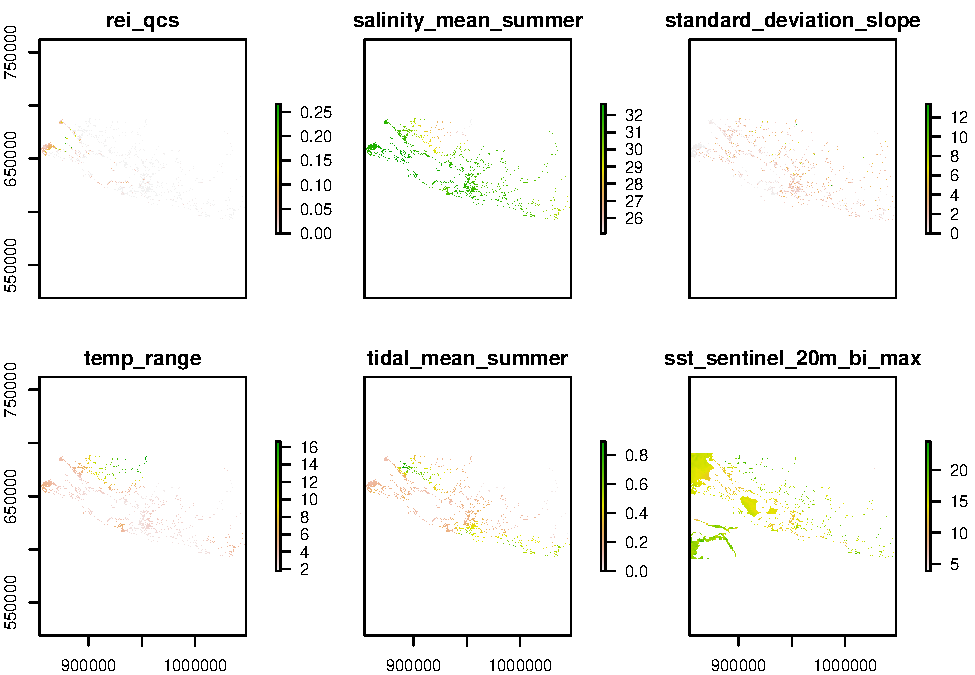
\includegraphics{C:/Data/Git/Broughton/Results/DFO_Class_Report_2024-09-14_files/figure-latex/unnamed-chunk-1-1.pdf}
\caption{Maps of the selected, unmodified predictors.}
\end{figure}

\begin{figure}
\centering
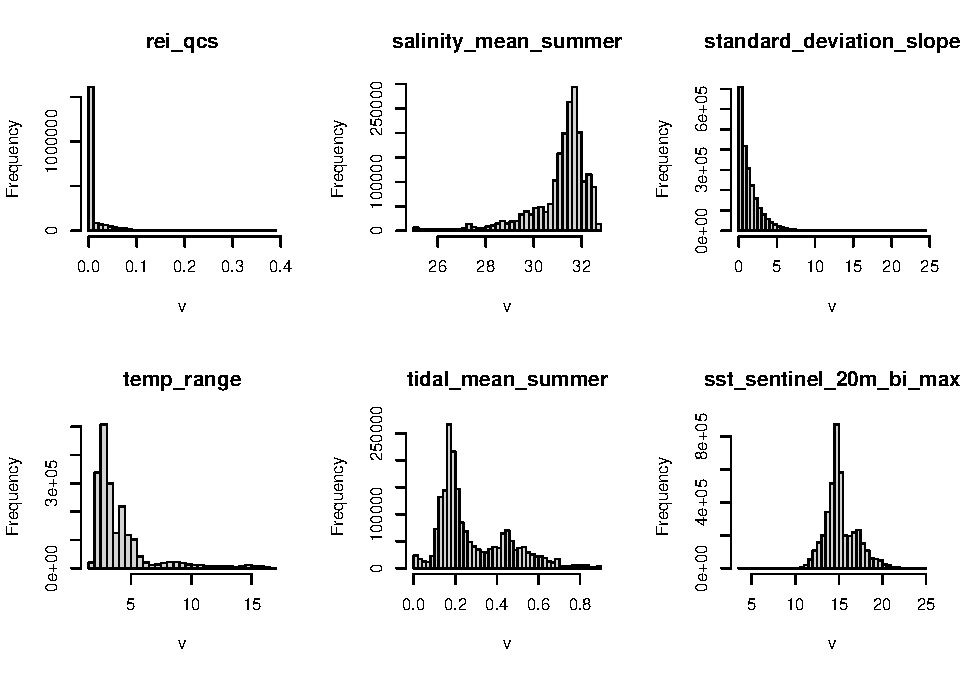
\includegraphics{C:/Data/Git/Broughton/Results/DFO_Class_Report_2024-09-14_files/figure-latex/unnamed-chunk-2-1.pdf}
\caption{Histograms of the selected, unmodified predictors.}
\end{figure}

\begin{figure}
\centering
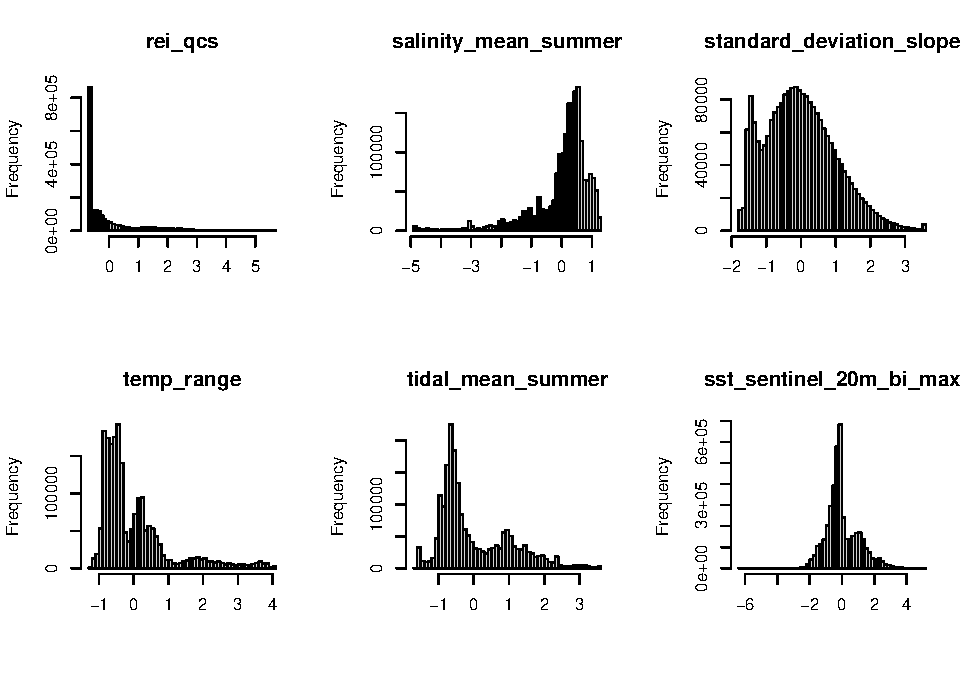
\includegraphics{C:/Data/Git/Broughton/Results/DFO_Class_Report_2024-09-14_files/figure-latex/FixedHists-1.pdf}
\caption{Histograms of selected, transformed and scaled predictor data.}
\end{figure}

\hypertarget{results}{%
\section{Results}\label{results}}

perhaps some words in here will help.

\hypertarget{part-1---cluster-number}{%
\subsection{Part 1 - Cluster number}\label{part-1---cluster-number}}

\begin{figure}
\centering
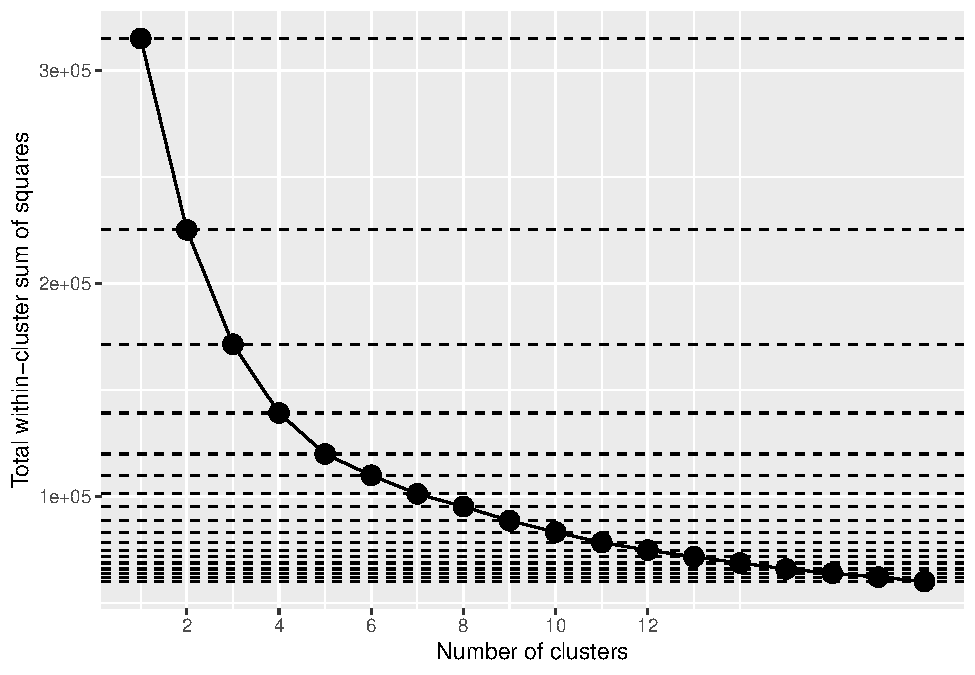
\includegraphics{C:/Data/Git/Broughton/Results/DFO_Class_Report_2024-09-14_files/figure-latex/Fig4_ScreePlot-1.pdf}
\caption{Scree plot showing the total within sum-of-squares across a
range of cluster numbers.}
\end{figure}

\begin{figure}
\centering
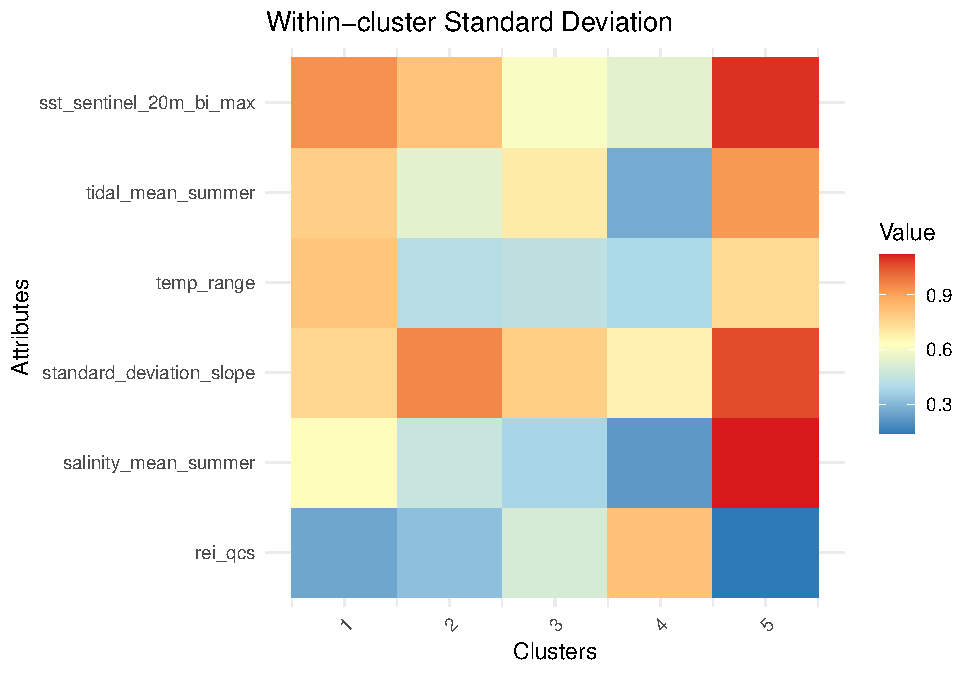
\includegraphics{C:/Data/Git/Broughton/Results/DFO_Class_Report_2024-09-14_files/figure-latex/HeatMap-1.pdf}
\caption{Heat map showing within cluster standard deviation of the
predictors.}
\end{figure}

\begin{figure}
\centering
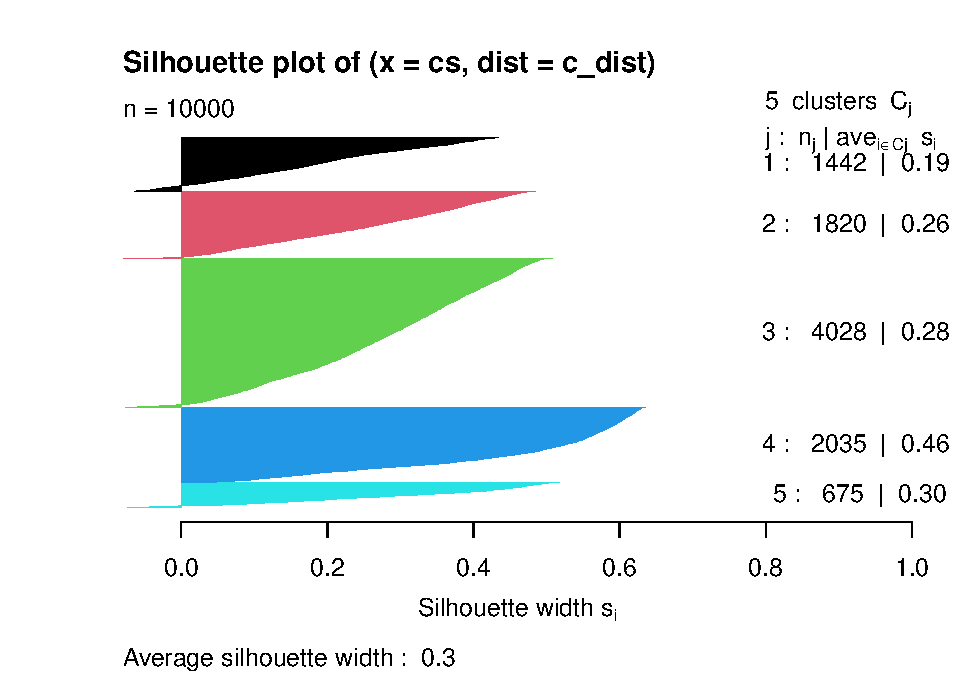
\includegraphics{C:/Data/Git/Broughton/Results/DFO_Class_Report_2024-09-14_files/figure-latex/SilhouettePlot-1.pdf}
\caption{Silhouette plot showing pixel membership in each cluster and
silhouette widths.}
\end{figure}

\hypertarget{part-2---clusters-and-predictor-loadings}{%
\subsection{Part 2 - Clusters and predictor
loadings}\label{part-2---clusters-and-predictor-loadings}}

First we do PCA plots and then we show loadings as violin plots. A table
of loadings should also be here.

\begin{figure}
\centering
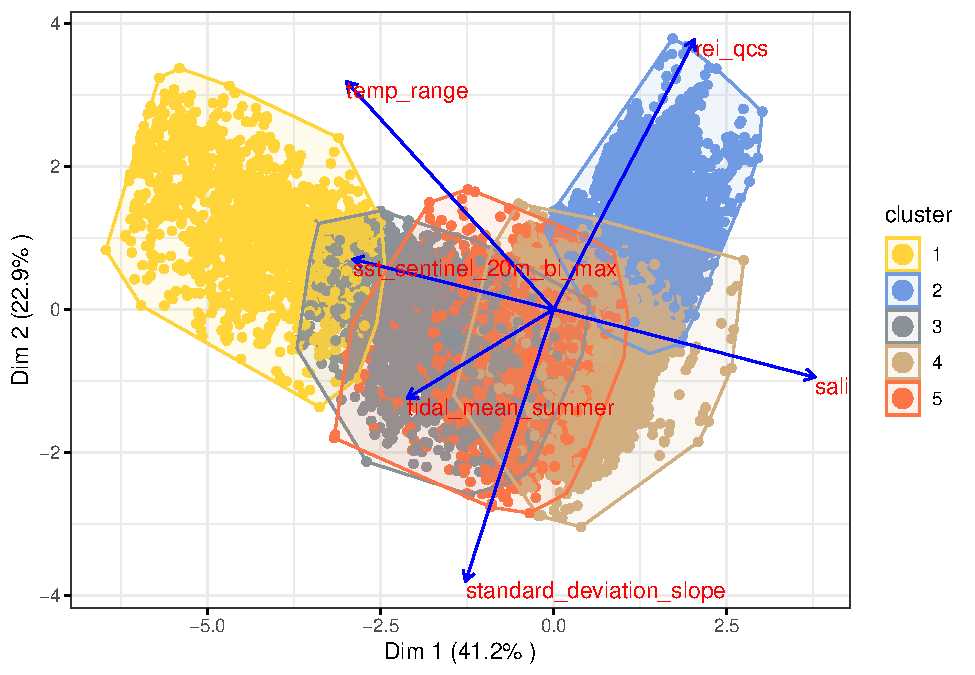
\includegraphics{C:/Data/Git/Broughton/Results/DFO_Class_Report_2024-09-14_files/figure-latex/Fig7_PCAPlot1-1.pdf}
\caption{PCA Plots showing the clusters across the first and second
dimensions.}
\end{figure}

Impressions of how the clusters are formed \ldots{}

\begin{table}
\centering
\caption{\label{tab:PCATable}Correlation matrix for assessing predictor cross-correlations}
\centering
\resizebox{\ifdim\width>\linewidth\linewidth\else\width\fi}{!}{
\begin{tabular}[t]{lrrrrrr}
\toprule
  & PC1 & PC2 & PC3 & PC4 & PC5 & PC6\\
\midrule
rei\_qcs & 0.3148978 & 0.5834475 & -0.1078770 & -0.3454116 & 0.6105640 & -0.2381037\\
salinity\_mean\_summer & 0.5835270 & -0.1470545 & 0.0979808 & 0.1948666 & 0.2503854 & 0.7263643\\
standard\_deviation\_slope & -0.1965297 & -0.5884746 & -0.4913184 & -0.4905704 & 0.3452325 & 0.1176227\\
temp\_range & -0.4625377 & 0.4928553 & -0.0526314 & -0.3309206 & -0.1831007 & 0.6303556\\
tidal\_mean\_summer & -0.3269805 & -0.1924344 & 0.8129287 & -0.1588818 & 0.4119965 & 0.0146690\\
\addlinespace
sst\_sentinel\_20m\_bi\_max & -0.4481677 & 0.1082785 & -0.2715611 & 0.6835983 & 0.4920024 & 0.0655979\\
\bottomrule
\end{tabular}}
\end{table}

Impressions of how the lower dimensions of the PCA contribute \ldots{}

\begin{figure}
\centering
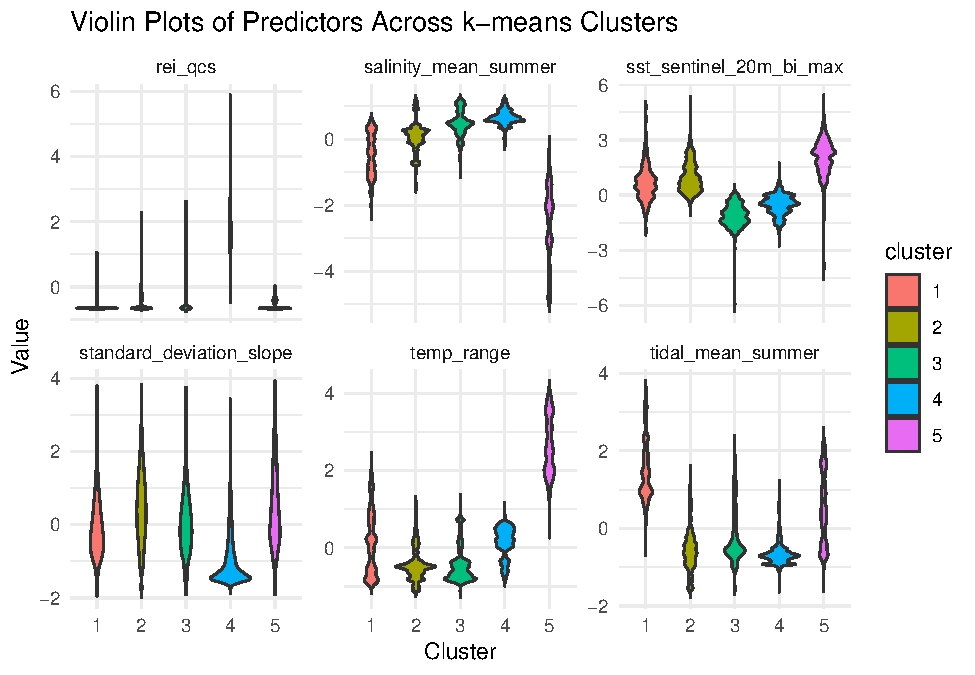
\includegraphics{C:/Data/Git/Broughton/Results/DFO_Class_Report_2024-09-14_files/figure-latex/ViolinPlot-1.pdf}
\caption{Violin plots showing distribiton of predictors in each of the
k-means clusters.}
\end{figure}

What beautiful violins.

\newpage

\hypertarget{addendums}{%
\section{Addendums}\label{addendums}}

\hypertarget{r-packages}{%
\subsection{R packages}\label{r-packages}}

dplyr: A fast, consistent set of tools for working with data frame like
objects, both in memory and out of memory.

ggplot2: A system for `declaratively' creating graphics based on ``The
Grammar of Graphics'`. You provide the data, tell 'ggplot2' how to map
variables to aesthetics, what graphical primitives to use, and it takes
care of the details. Hmisc: Contains many functions useful for data
analysis, high-level graphics, utility operations, functions for
computing sample size and power, simulation, importing and annotating
datasets, imputing missing values, advanced table making, variable
clustering, character string manipulation, conversion of R objects to
LaTeX and html code, and recoding variables. Used here to add standard
deviation to as lines to ggplot.

knitr: Provides a general-purpose tool for dynamic report generation in
R using Literate Programming techniques. Used here for Markdown
formatting as html or pdf.

lubridate : Functions to work with date-times and time-spans: fast and
user friendly parsing of date-time data, extraction and updating of
components of a date-time (years, months, days, hours, minutes, and
seconds), algebraic manipulation on date-time and time-span objects.
Used here to pool dates to month.

markdown: R Markdown allows the use of knitr and Pandoc in the R
environment. This package translates R Markdown to standard Markdown
that knitr and Pandoc render to the desired output format (e.g., PDF,
HTML, Word, etc).

purrr: A complete and consistent functional programming toolkit for data
manupulation in R.

readxl: Imports excel files into R.

reshape2: Flexibly restructure and aggregate data using just two
functions: melt and `dcast'. Used here for ggplot() support.

tibble: Functions for manipulating the tibble data format in R. Used
here for the deframe() function.

vegan: Ordination methods, diversity analysis and other functions for
community and vegetation ecologists.

\end{document}
